\chapter{Primera aproximación a una métrica apropiada. Distancia de Levenshtein}
\label{ch:Levenshtein}

\lettrine[lraise=-0.1, lines=2, loversize=0.2]{L}{a} distancia de Levenshtein
recibe su nombre del científico ruso Vladimir Levenshtein, quién la creó en 1965.

% Definir la distancia de Levenshtein original (citarlo bien)
\vspace{0.3cm}
\textit{"La distancia de Levenshtein, distancia de edición o distancia entre
palabras es el número mínimo de operaciones requeridas para transformar una cadena
de caracteres en otra"}.
\vspace{-0.2cm}
{\flushleft{\hfill \emph{- Wikipedia, 2020, párrafo 1,} \cite{Wikipedia}}}
\vspace{0.3cm}

% Explicar la modificación realizada para adaptarlo a nuestro caso
Aunque este algoritmo esté concebido como métrica de la diferencia entre dos
cadenas de caracteres, podemos aplicar el concepto básico a dos salidas de la
campaña de inyección de fallos. Redefiniendo la distancia de Levenshtein para
nuestro caso en particular:

\vspace{0.3cm}
\textit{"La distancia de Levenshtein es el número mínimo de bits que hay que
conmutar de la salida de una campaña de inyección de fallos para transformarla 
en otra"}.
\vspace{0.3cm}

Existe una operación lógica ya mencionada anteriormente que permite comparar dos
salidas obteniendo como resultado ceros para aquellos bits en los que son iguales
y unos en los diferentes. La operación \textit{XOR} bit a bit permite obtener
tantos unos como diferencias existen entre las dos salidas. La distancia de
levenshtein entre dos salidas de una campaña es el sumatorio de todos estos bits 
con valor lógico alto.

% Comentar la hipótesis realizada para diagnosticar en base a esto
    % Si el SEU se encuentra en el diccionario -> levenDist = 0
    % Si el SEU no se encuentra en el diccionario -> min(levenDist) será el más
    % cercano
De esta forma, según la hipótesis inicial \ref{hyp:inicial}, dos \gls{SEU}
que estén próximos entre sí tendrán una distancia de Levenshtein relativamente
baja entre ellos. Cuando el diccionario de fallos contiene el error lógico a
diagnosticar, existirá al menos una entrada con la cual la distancia de
Levenshtein será cero. Cuando esto sucede, damos al diagnóstico por terminado,
aunque en el capítulo \ref{ch:CampanasIterativas} veremos una ampliación de la 
técnica que permite continuar un poco más y aumentar la confianza en los 
resultados obtenidos. En caso contrario, las entradas a menor distancia del run a
diagnosticar (de aquí en adelante \textit{"target run"}) serán utilizadas para
localizarlo.


\section{Elaboración de la base de datos de distancias}
\label{sec:LevenDist}
% Explicar como se calculan las distancias de Leven y como se almacenan en memoria
Antes de explicar más concretamente cómo se calculan las distancias entre runs del
diccionario y se elabora la tabla de distancias, es necesario comentar cómo está
expresada inicialmente la información de las salidas una vez son comparadas con el
\textit{Golden run} (ver figura \ref{fig:PostprocesadoSalida}). Un detalle hasta 
ahora no mencionado es que el diccionario se divide en dos archivos,
\textit{"damages.csv"} e \textit{"injections.csv"}. Cada run divide su información
entre estos dos ficheros, ubicando ciclo y \gls{FF} de la inyección en 
\textit{injections.csv} y los errores que esta genera a la salida del circuito, en
\textit{"damages.csv"}.
Para explicar como está dispuesta la información dentro de este último documento 
vamos a suponer que el \gls{CUT} tiene 8 salidas y cada ejecución de la campaña 
dura 10 ciclos de reloj. Un ejemplo de salida contenida en el diccionario de este
circuito puede ser:

\begin{center}
    0:1A,3:C0,4:80,7:1E,8:1C,9:02
\end{center}

% Hex -> binario almacenado como enteros -> XOR bit a bit -> sumatorio de 1s
Cada pareja de números separados por dos puntos significan
\textit{"Ciclo:Fallos"}, donde \textit{Fallos} es una representación hexadecimal
de las salidas del \gls{CUT} en el ciclo \textit{Ciclo}. Los fallos de distintos 
ciclos están separados entre sí mediante comas, y cada run contenido en el 
diccionario se encuentra en una línea independiente. Podemos observar en el 
ejemplo anterior que ciertos ciclos no aparecen. Estos son los ciclos de la 
ejecución donde la salida no presenta discrepancias con el \textit{Golden run}. 
De esta forma, las inyecciones que no generen fallos a la salida del circuito se 
corresponderán con líneas vacías del diccionario.

Ahora que conocemos cómo está contenida la información en el diccionario de
fallos, podemos proceder al cálculo de las distancias. El primer paso es leer la
información de ambos archivos y cargarlos en memoria, rellenando los ciclos sin
fallos con ceros. Hemos decidido almacenar la información en forma de enteros 
en base 10, aunque estos sean tratados como binario. A contiuación se realiza, bit
a bit, la \textit{XOR} de cada run con el resto. Como último paso en el cálculo de
las distancias de Levenshtein, se toman los resultados de la operación lógica y se
suman los bits con valor lógico alto. El resultado de esta suma es la distancia
en cuestión.

% Imagen 1: De HEX a binario -> XOR con otro run -> sumatorio -> distancia
\begin{figure}[htbp]
    \centering
    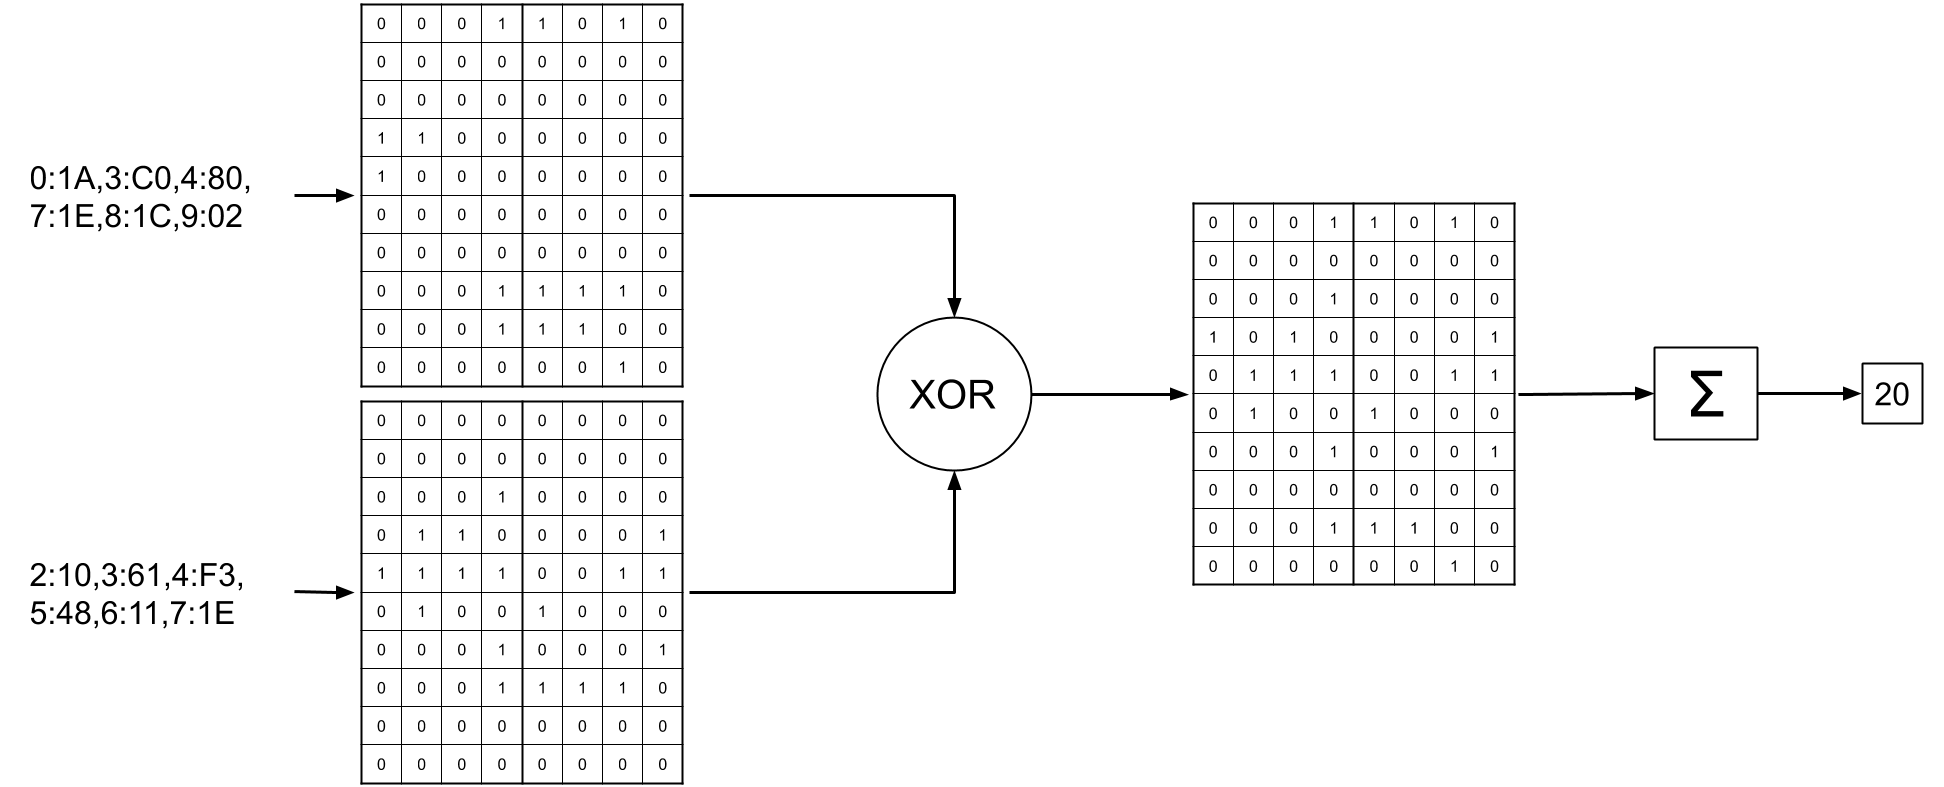
\includegraphics[width=0.95\linewidth]
    {Levenshtein/figuras/fig_1.png}
    \caption{Cálculo de la distancia de Levenshtein}
    \label{fig:LevenDist}
\end{figure}

% Esto para cada entrada del diccionario -> se obtiene tabla simetrica de
% distancias respecto a la diagonal.
Podemos elaborar una lista con las distancias entre el \textit{target run} y 
todas las entradas del diccionario de forma que la componente \textit{"i"} sea 
la distancia de Levenshtein entre el \gls{SEU} a diagnosticar y la entrada 
\textit{"i"}. Acompañando a esta lista tendríamos otra en la que se encuentra la
información de las inyecciones. 

Por último, notar que al tratarse de distancias, se cumplen las propiedades
típicas de una distancia: 
\begin{center}
    \textit{D(i,i) == 0}

    \textit{D(i,j) == D(j,i)}
\end{center}

\section{Diagnóstico basado en la distancia de Levenshtein}
\label{sec:LevenCands}
% Explicar cómo se seleccionan los candidatos en base a las distancias calculadas
% y por qué se selecciona de esa manera y no de otra. En one note hay apuntes de
% esto
Una vez hayamos calculado las distancias de Levenshtein entre el \textit{target
run} y todas las entradas del dicionario y hayamos elaborado las dos listas
mencionadas tendremos todo lo necesario para llevar a cabo el diagnóstico con esta
primera versión de la técnica.

Inicialmente, la selección de los candidatos %...  ecuacion del porcentaje
%... la version final... ordenar y coger los n primeros
% candidato/candidato definitivo


\section{Resultados experimentales}
\label{sec:LevenResults}


\subsection{Diccionarios exhaustivos}
\label{subsec:LevDicExhaust}
% Siempre aparece mínimo el correcto, a veces más debido a colisiones


\subsection{Diccionarios no exhaustivos}
\label{subsec:LevDicNoExhaust}


\endinput
